\chapter{Аналитическая часть}

В данном разделе будут описаны основные теоретические аспекты, необходимые для решения поставленной задачи.

\section{Модель гауссовой смеси}

При решении задач машинного обучения зачастую необходимо каким-то образом представлять данные. Самый простой способ --- взять сами точки как представление данных (пример представлен на рисунке \ref{fig:data}). Однако этот подход может оказаться бесполезным, если набор данных огромен или если есть необходимость в представлении характеристик данных. При оценке плотности данные представляются компактно, используя функцию плотности из некоторого параметрического семейства, например гауссово или бета-распределение. Также можно рассчитывать среднее значение и дисперсию рассматриваемого набора данных, чтобы компактно представить его с использованием распределения Гаусса. Затем можно использовать параметры этого распределения (среднее значение и дисперсию) для его визуализации, полагая, что оно лежит в основе данных. Иначе говоря, делается предположение о том, что набор данных является реализацией выбранного распределения.~\cite{math}

На практике распределение Гаусса имеет ограниченные возможности моделирования. Например, гауссово приближение плотности, сгенерировавшее данные на рисунке \ref{fig:data}, было бы неточным приближением. Далее будет рассмотрено более выразительное семейство распределений, которое можно использовать для оценки плотности данных --- модели смеси. Модели смесей могут использоваться для описания распределения $p(x)$ выпуклой комбинацией $K$ простых (базовых) распределений.~\cite{math}
\begin{equation}
	p(x) = \sum_{k=1}^{K}\pi_k p_k(x); 0 \leq \pi_k \leq 1; \sum_{k=1}^{K}\pi_k = 1,
\end{equation}
где компоненты $p_k$ являются членами семейства базовых распределений, например Гаусса, Бернулли или гамма-распределение, а $\pi_k$ --- веса смеси. Модели смесей более выразительны, чем соответствующие базовые распределения, поскольку они допускают мультимодальные представления данных, то есть они могут описывать наборы данных с несколькими <<кластерами>>, как в примере на рисунке \ref{fig:data}.~\cite{math}

\begin{figure}[H]
	\centering
	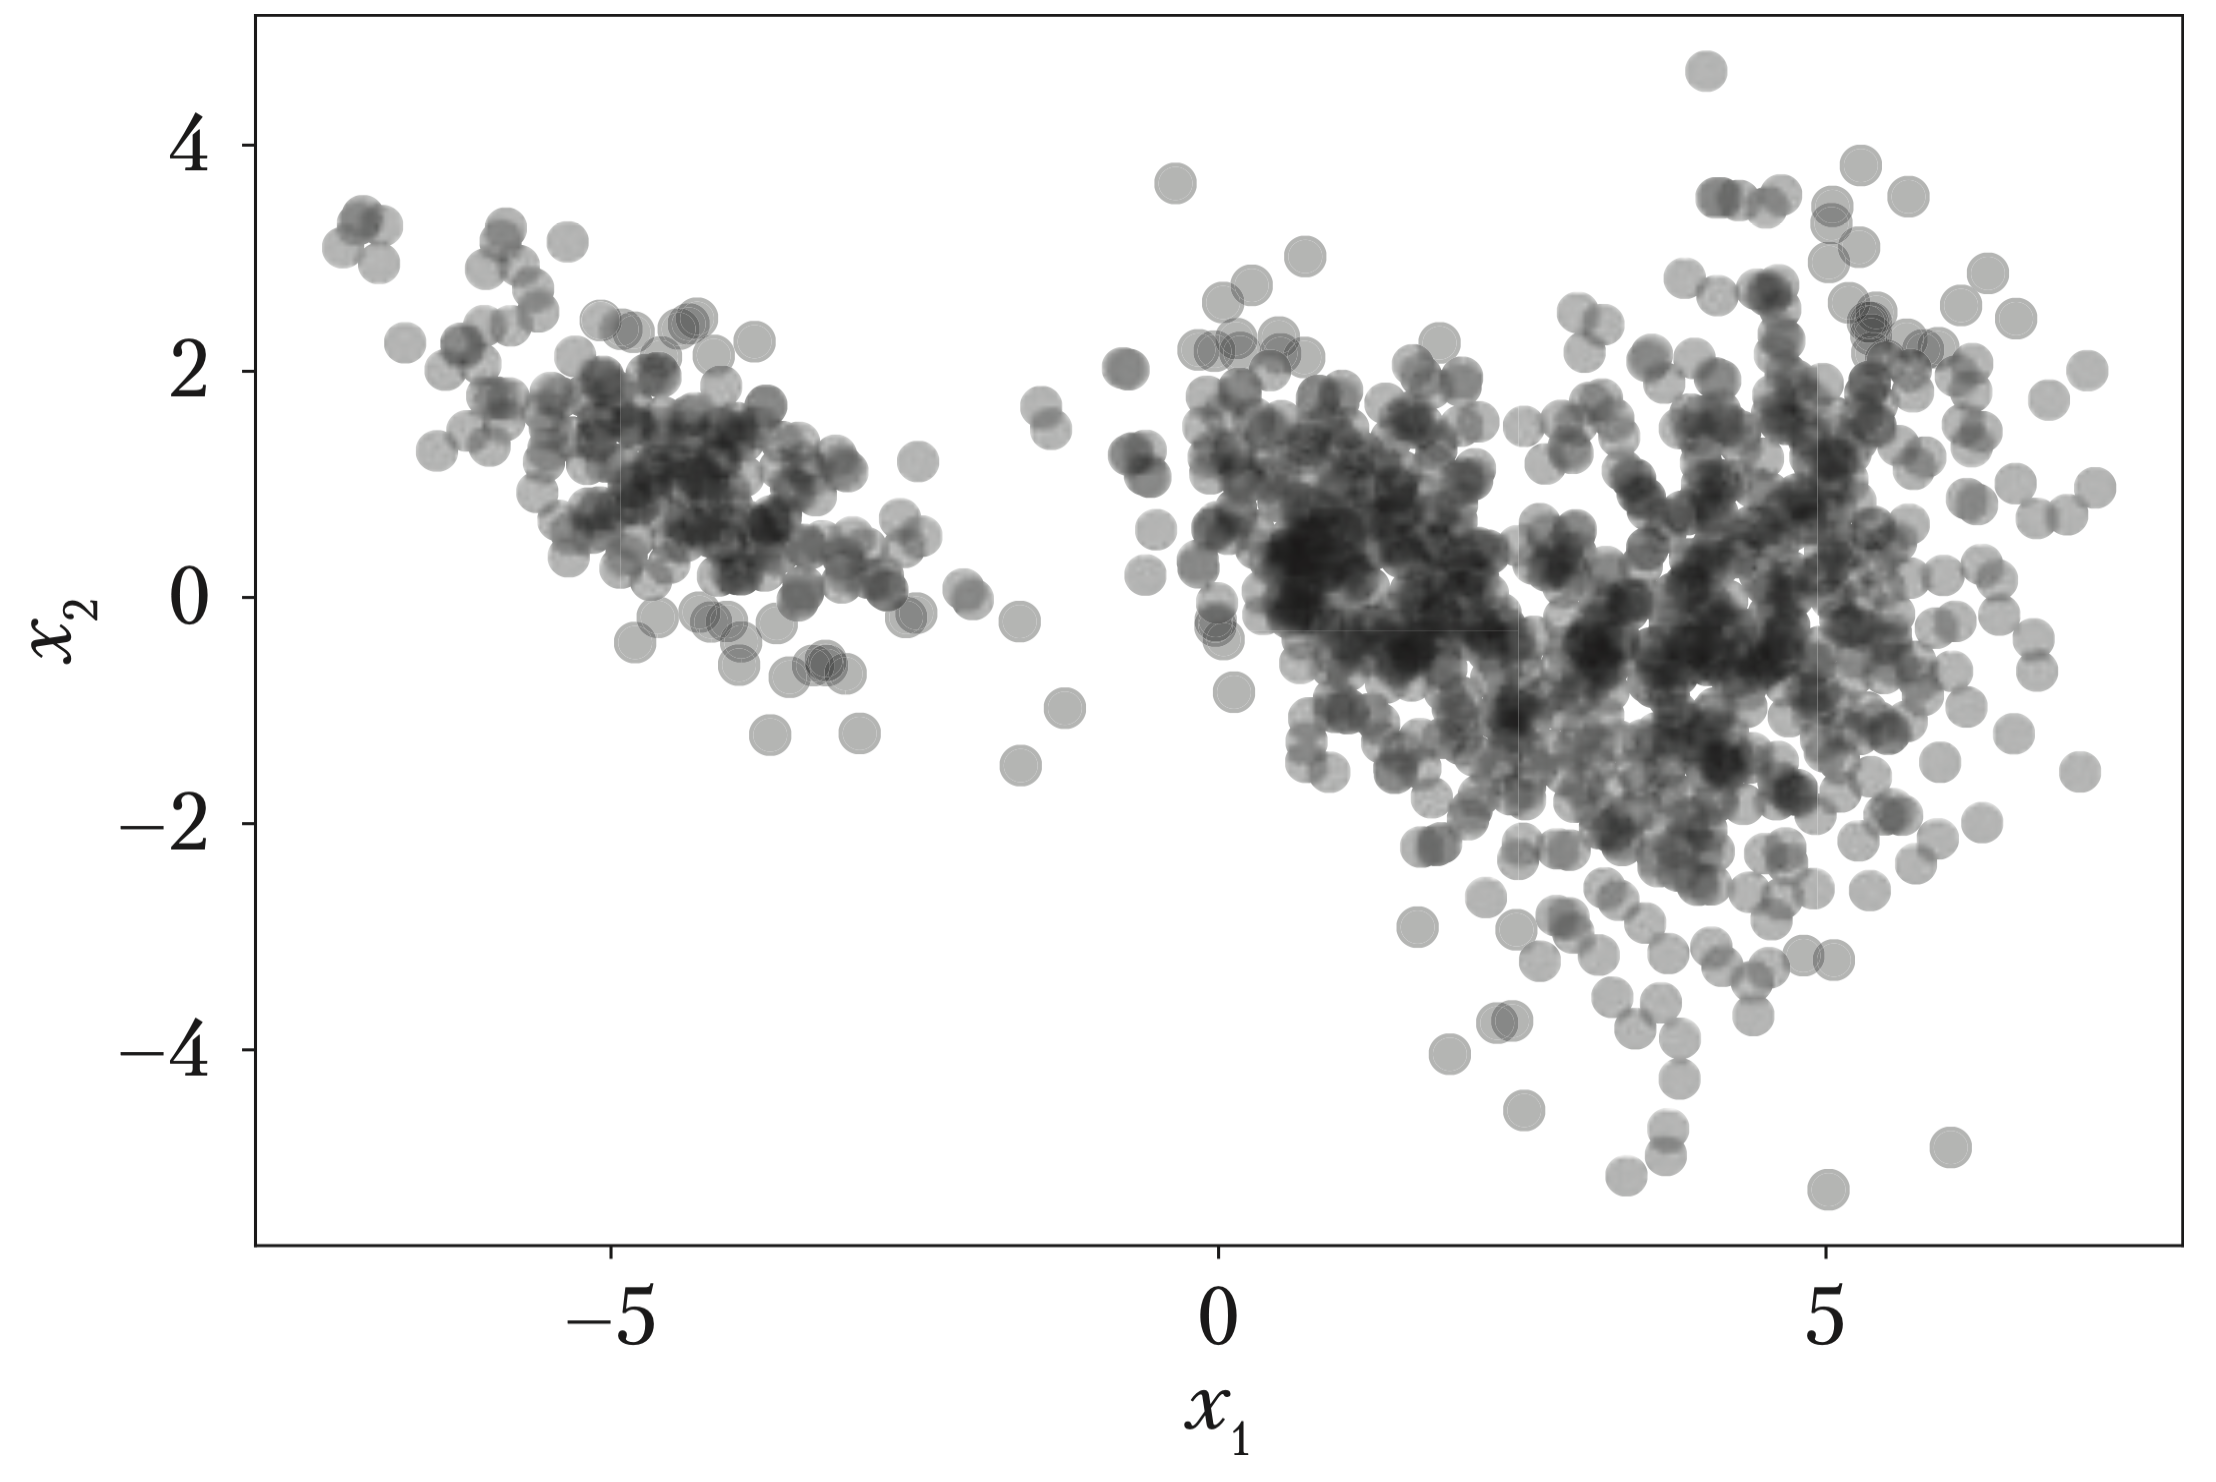
\includegraphics[width=0.8\textwidth]{assets/data.png}
	\caption{Двумерный набор данных, который не может быть осмысленно представлен с помощью гауссиана}
	\label{fig:data}
\end{figure}

Рассмотрим модели гауссовой смеси (Gaussian mixture models~---~GMM), где базовые распределения являются гауссианами. При построении смеси для исходного набора данных необходимо стремиться к максимизации вероятности параметров модели для обучения GMM. Однако в отличие от других приложений для представления данных (таких, как линейная регрессия или PCA), нельзя найти максимум функции правдоподобия в явной форме. Вместо этого предлагается система уравнений, которую можно решить только итерационно.~\cite{math}

Модель гауссовой смеси (Gaussian mixture model, GMM) --- это модель плотности, в которой комбинируется конечное число $K$ гауссовых распределений $N(x \vert \mu_k, \Sigma_k)$, так чтобы
\begin{equation}
	p(x \vert \theta) = \sum_{k=1}^{K}\pi_k N(x \vert \mu_k, \Sigma_k); 0 \leq \pi_k \leq 1; \sum_{k=1}^{K}\pi_k = 1,
\end{equation}
где $\theta := {\mu_k, \Sigma_k, \pi_k : k = 1, ..., K}$ является представлением совокупности всех параметров модели. Эта выпуклая комбинация распределений Гаусса даёт значительно большую гибкость при моделировании сложных многомерных плотностей, чем простое гауссово распределение.~\cite{math} На рисунке \ref{fig:gmm} показаны взвешенные компоненты и плотность смеси, которая представлена как
\begin{equation}
	p(x \vert \theta) = 0.5N(x \vert -2, \frac{1}{2}) + 0.2N(x \vert 1, 2) + 0.3N(x \vert 4, 1).
\end{equation}

\begin{figure}[H]
	\centering
	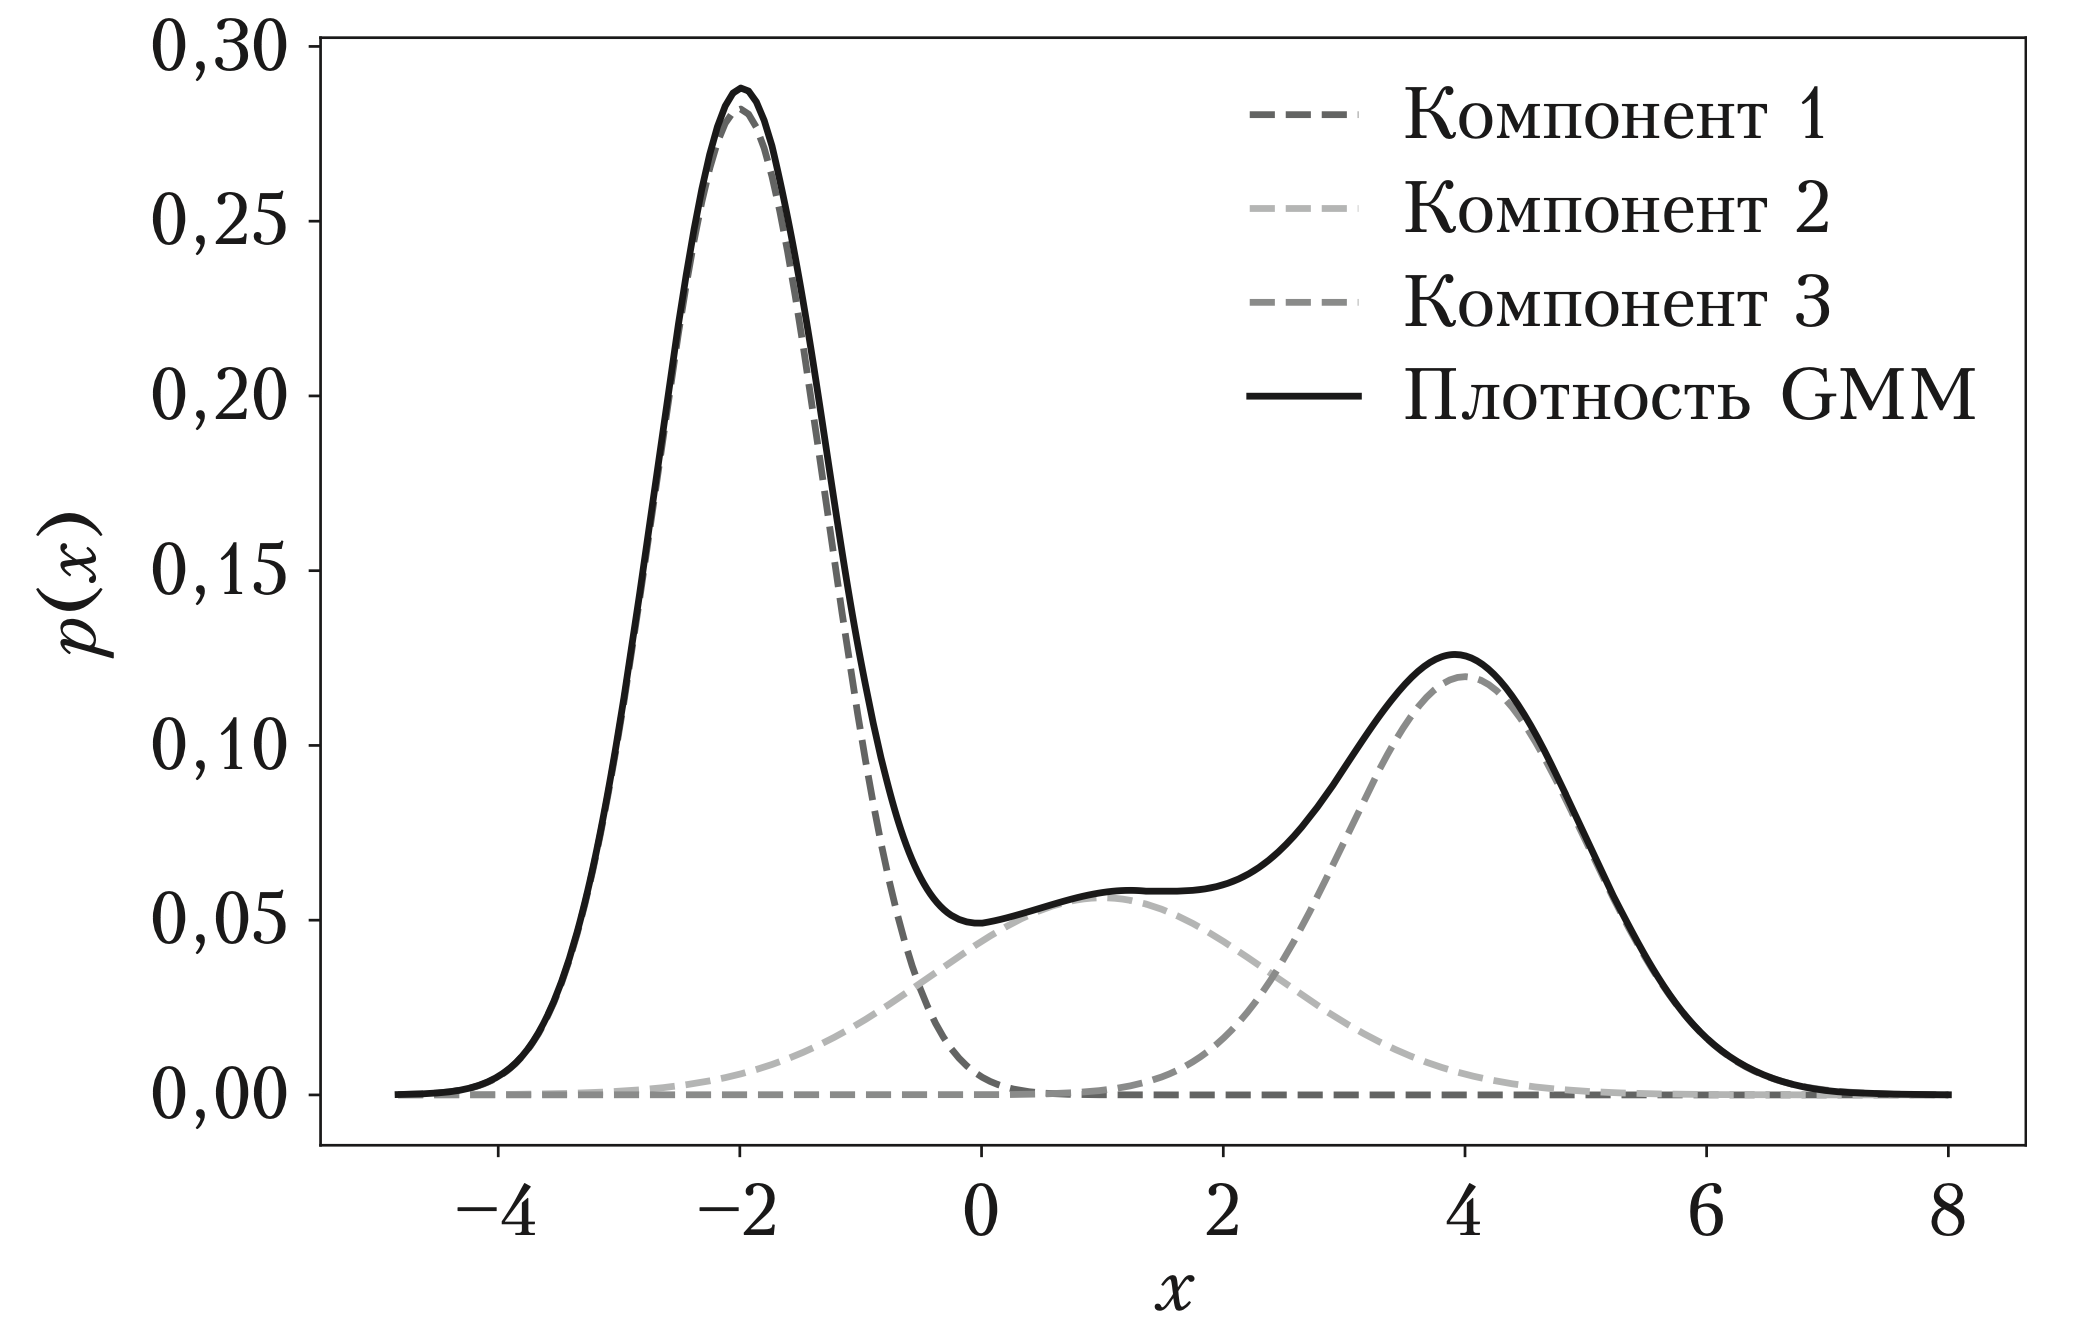
\includegraphics[width=0.8\textwidth]{assets/gmm.png}
	\caption{Модель	гауссовой смеси, которая представляет собой выпуклой комбинацией распределений Гаусса и является более выразительной, чем любой отдельный её компонент}
	\label{fig:gmm}
\end{figure}

Предположим, нам имеется набор данных $X = {x_1, \dots, x_N}$, где $x_n$, $n = 1, \dots, N$, взяты независимыми и одинаково распределёнными из неизвестного распределения $p(x)$. Наша цель --- найти наиболее точное приближение/представление этого неизвестного распределения $p(x)$ с помощью GMM с $K$ компонентов смеси. Параметрами GMM являются $K$-средние $\mu_k$, ковариации $\Sigma_k$ и веса смеси $\pi_k$. Все эти свободные параметры суммируются в $\theta := {\pi_k, \mu_k, \Sigma_k : k = 1, ..., K}$.~\cite{math}

Далее будет подробно описана методика получения оценки максимального правдоподобия $\theta_{ML}$ параметров модели $\theta$.~\cite{math} Начнём с записи вероятности, то есть прогнозируемого распределения обучающего набора данных. Для этого запишем факторизованную вероятность для независимых и одинаково распределённых случайных величин
\begin{equation}
	p(X \vert \theta) = \prod_{n=1}^{N}p(x_n \vert \theta),\ p(x_n \vert \theta) = \sum_{k=1}^{K}\pi_k N(x_n \vert \mu_k, \Sigma_k),
\end{equation}
где каждый член вероятности $p(x_n \vert \theta)$ является функцией плотности гауссовой смеси. Тогда можно определить логарифмическое правдоподобие как
\begin{equation}\label{eq:theta}
	\log p(X \vert \theta) = \sum_{n=1}^{N}\log p(x_n \vert \theta) = \sum_{n=1}^{N}\log \sum_{k=1}^{K}\pi_k N(x_n \vert \mu_k, \Sigma_k).
\end{equation}

Далее необходимо найти значения параметров, которые максимизируют логарифмическое правдоподобие $\theta*_{ML}$, определённое в (\ref{eq:theta}). Затем можно вычислить градиент $dL/d\theta$ логарифма правдоподобия относительно параметров модели $\theta$, приравнять его к нулю и решить относительно $\theta$. Однако в данном случае для рассматриваемой оценки максимального правдоподобия, нельзя получить решение в явной форме. Тем не менее, можно использовать итерационную схему, чтобы с достаточной точностью найти параметры модели $\theta_{ML}$. Ключевая идея состоит в том, чтобы обновлять один параметр модели за одну итерацию, оставляя другие параметры неизменными.~\cite{math}

Определяем количество
\begin{equation}\label{eq:r}
 	r_{nk} := \frac{\pi_k N(x_n \vert \mu_k, \Sigma_k)}{\sum_{j=1}^{K}\pi_j N(x_n \vert \mu_j, \Sigma_j)}
\end{equation}
как ответственность $k$-го компонента смеси за $n$-ю точку данных. Ответственность $r_{nk}$ $k$-го компонента смеси для точки данных $x_n$ пропорциональна правдоподобию
\begin{equation}
	p(x_n \vert \pi_k, \mu_k, \Sigma_k) = \pi_k N(x_n \vert \mu_k, \Sigma_k)
\end{equation}
компонента смеси с учётом параметров точки исходных данных\footnote{$r_n$ следует распределению Больцмана-Гиббса.}. Следовательно, компоненты смеси
несут большую ответственность за точку данных, когда точка данных допустима для конкретного компонента смеси. Стоит отметить, что
$r_n : = [r_n1, \dots, r_{nK}]^T \in \mathbb{R}_k$ является нормированным вектором вероятности, то есть
$\Sigma_k r_{nk} = 1 \ge 0$. Этот вектор вероятности распределяет вероятностную массу
между $K$ компонентами смеси, и можно рассматривать $r_n$ как <<мягкое присвоение>> $x_n$ компонентам $K$ смеси. Следовательно, ответственность $r_{nk}$ из (\ref{eq:r})
представляет собой вероятность того, что $x_n$ был сгенерирован $k$-м компонентом
смеси\footnote{Ответственность $r_{nk}$ --- это вероятность того, что $k$-й компонент смеси сгенерировал $n$-ю точку данных.}.~\cite{math}

Далее будет дано определение обновления параметров модели $\mu_k, \Sigma_k, \pi_k$ для заданных ответственностей. Будет показано, что все уравнения обновления зависят от ответственностей, что делает невозможным решение задачи оценки максимального правдоподобия в явном виде. Однако для имеющихся ответственностей можно обновлять один параметр модели за один шаг, оставляя другие неизменными. После этого должен производиться пересчёт ответственности. Итерация этих двух шагов в конечном итоге приведёт к локальному оптимуму и является конкретным воплощением алгоритма EM.~\cite{math}

Обновление средних параметров GMM $\mu_k, k = 1, \dots, K$, определяется выражением
\begin{equation}\label{eq:mu}
	\mu_k^{new} = \frac{\sum_{n=1}^{N}r_{nk}x_n}{\sum_{n=1}^{N}r_{nk}},
\end{equation}
где ответственности $r_{nk}$ определены в (\ref{eq:r}).~\cite{math}

Обновление параметров ковариации $\Sigma_k, k = 1, ..., K$, GMM определяется выражением
\begin{equation}\label{eq:sigma}
	\Sigma_k^{new} = \frac{1}{N_k}\sum_{n=1}^{N}r_{nk}(x_n - \mu_k)(x_n - \mu_k)^T; N_k = \sum_{n=1}^{N}r_{nk},
\end{equation}
где $r_{nk}$ определены в (\ref{eq:r}) соответственно.~\cite{math}

Вес смеси GMM обновляется как
\begin{equation}\label{eq:pi}
	\pi_k^{new} = \frac{N_k}{N}, k = 1, \dots, K,
\end{equation}
где $N$ --- количество точек данных, а $N_k$ определено в (\ref{eq:sigma}).~\cite{math}

Можно определить вес смеси в (\ref{eq:pi}) как отношение общей ответственности $k$-го кластера к количеству точек данных. Поскольку $N = \Sigma_k N_k$, количество точек данных также можно интерпретировать как общую ответственность всех компонентов смеси вместе, так что $\pi_k$ --- относительная важность $k$-го компонента смеси для набора данных.~\cite{math}



\section{Оценка плотности ядра}

Оценка плотности ядра (Kernel density estimation, KDE)~\cite{rosenblatt, parzen}, является непараметрическим способом оценки плотности. Учитывая $N$ независимых и одинаково распределённых выборок, оценщик плотности ядра представляет лежащее в основе распределение как
\begin{equation}
	p(x) = \frac{1}{Nh}\sum_{n=1}^{N}k(\frac{x-x_n}{h}),
\end{equation}
где $k$ --- функция ядра, то есть неотрицательная функция, которая интегрируется до 1, а $h$ > 0 --- свободный параметр сглаживания полосы пропускания (bandwidth), который играет такую же роль, как размер ячейки в гистограммах. Пример зависимости вида гистограммы рассматриваемой случайной величины от различных значений параметра $h$ представлен на рисунке \ref{fig:kde-h}.~\cite{math}

\begin{figure}[H]
	\centering
	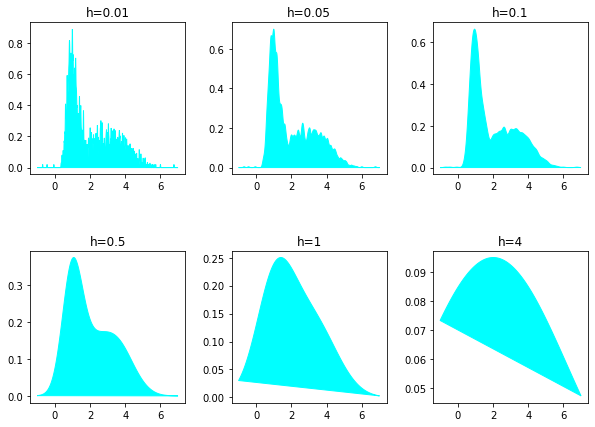
\includegraphics[width=\textwidth]{assets/kde-h.png}
	\caption{Пример зависимости вида гистограммы от различных значений параметра $h$}
	\label{fig:kde-h}
\end{figure}

Стоит отметить, что ядро помещается в каждую точку данных $x_n$ в наборе данных. Обычно используемые ядерные функции --- это равномерное распределение и распределение Гаусса. Также могут использоваться однородная, треугольная, бивзвешенная, тривзвешенная, Епанечникова, нормальная и другие ядерные функции.~\cite{math}

Оценки плотности ядра тесно связаны с гистограммами, однако по сравнению с ними у появляется возможность выбирать подходящее ядро, чтобы варьировать оценки плотности. На рисунке \ref{fig:kde} показана разница между гистограммой и оценкой плотности ядра (с ядром в форме Гаусса) для некоторого набора данных из 250 точек данных.~\cite{math}

\begin{figure}[H]
	\centering
	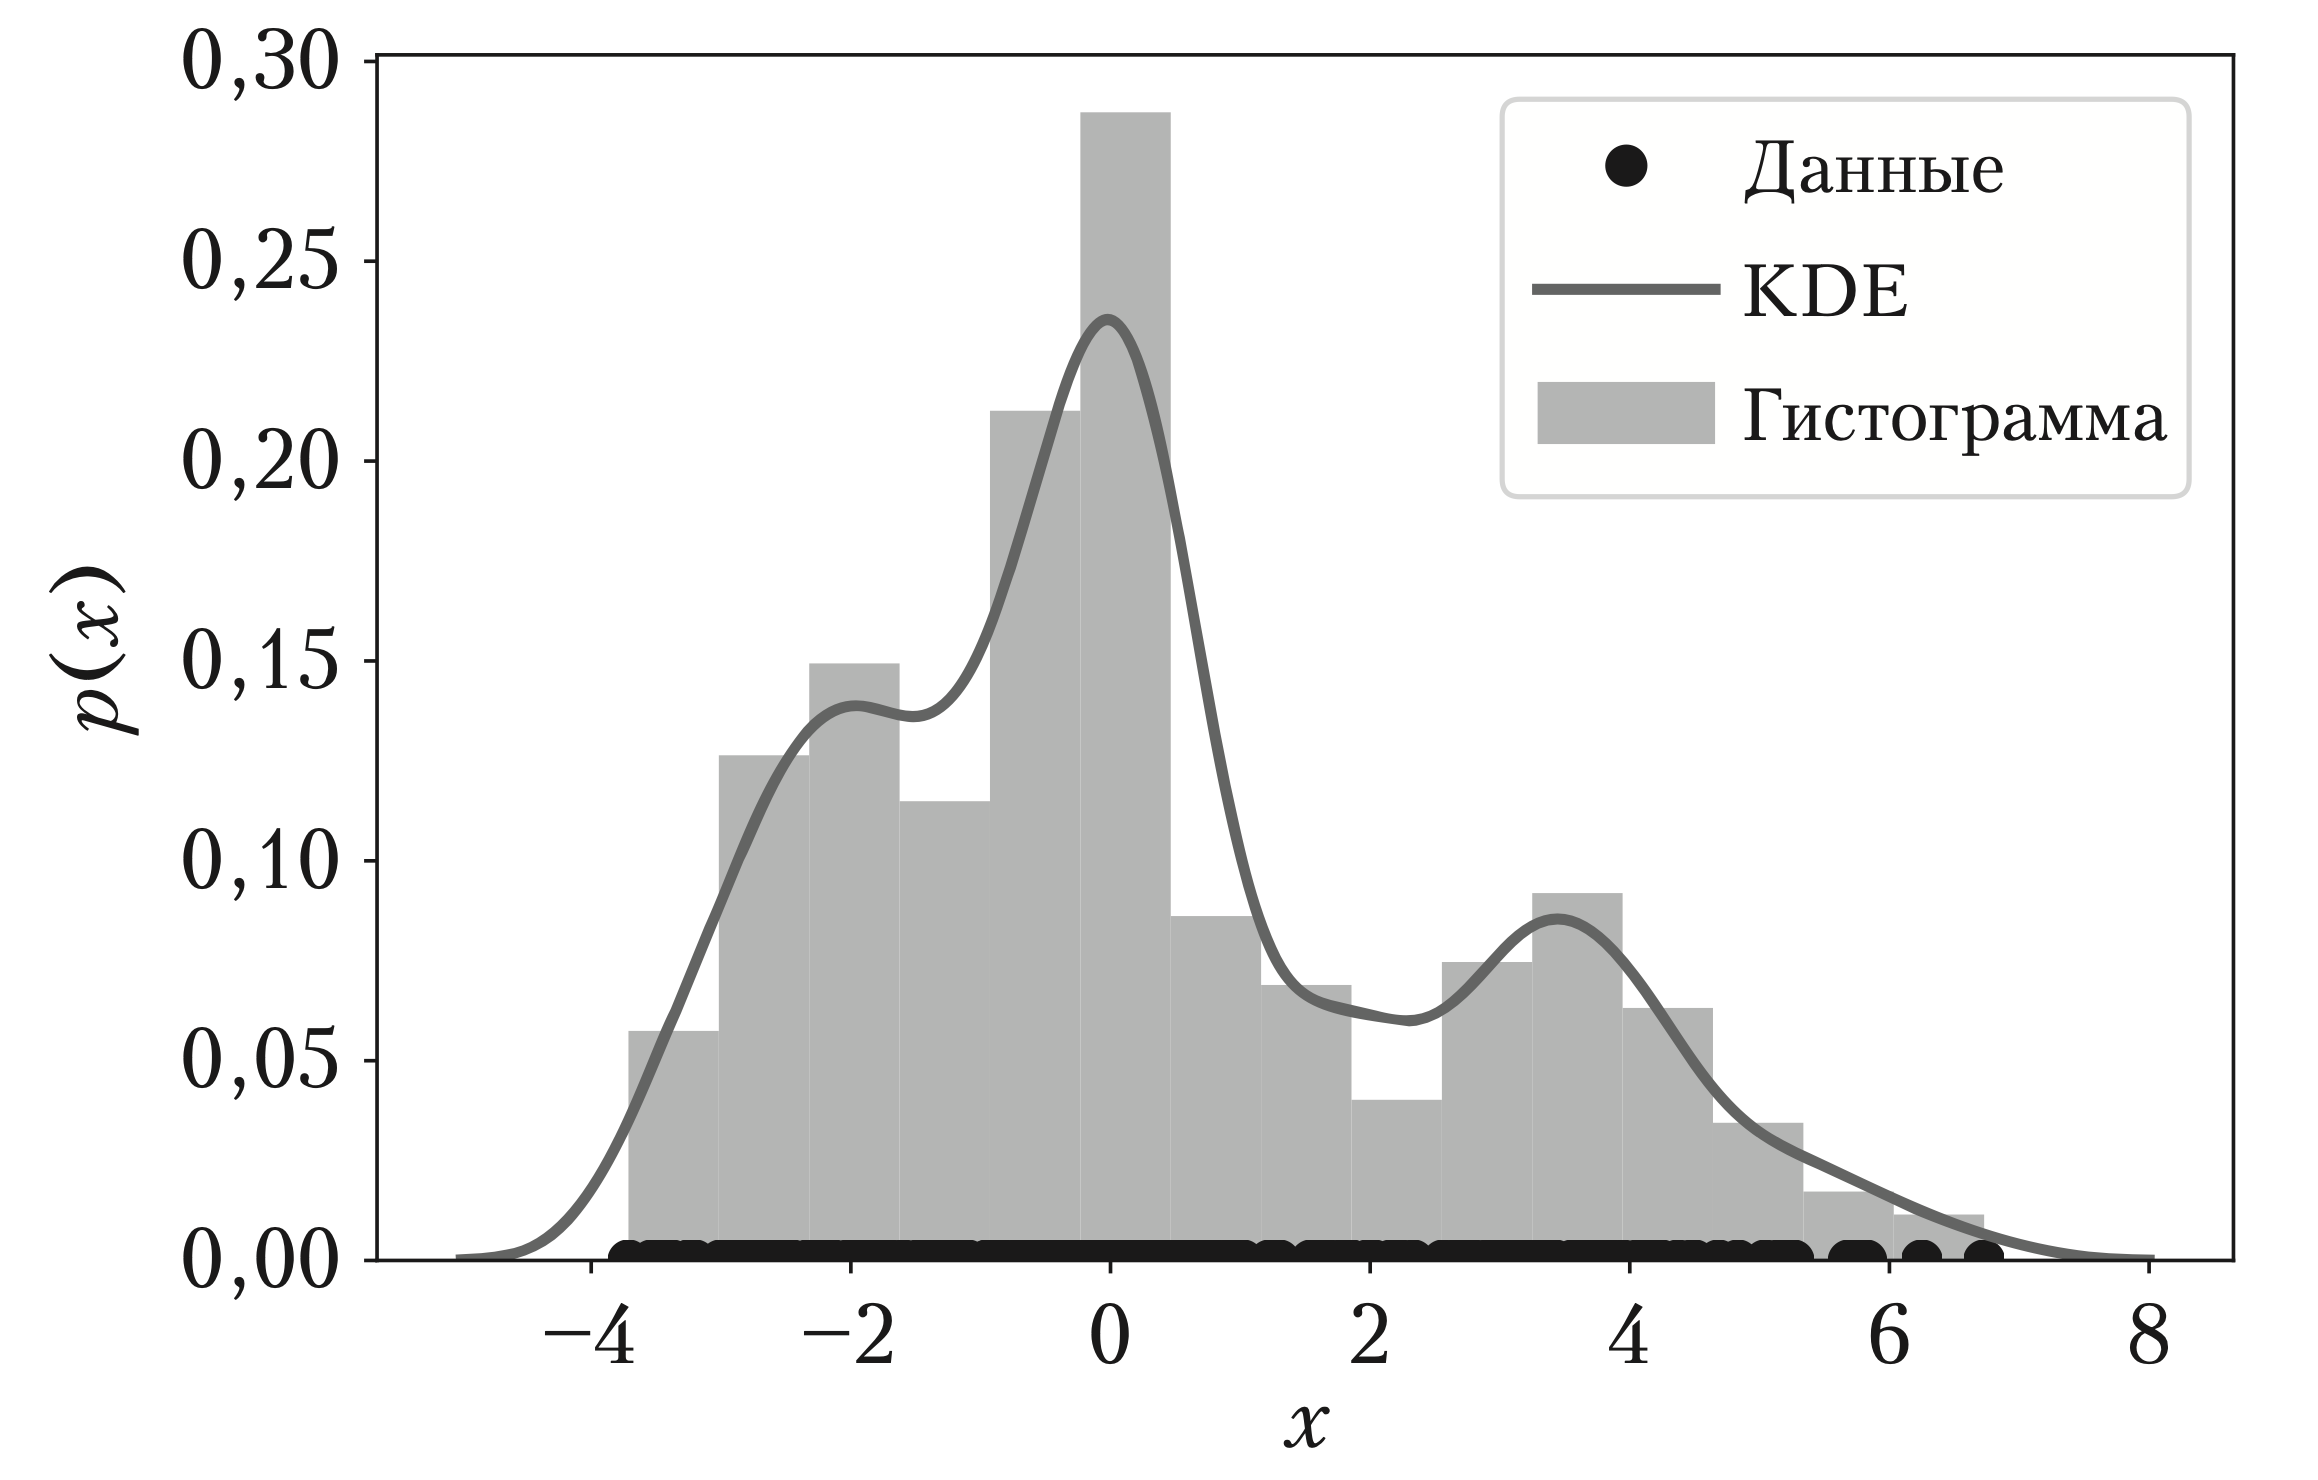
\includegraphics[width=0.8\textwidth]{assets/kde.png}
	\caption{Пример сравнения гистограммы и KDE}
	\label{fig:kde}
\end{figure}



\section{Вывод}

В данном разделе были рассмотрены модели гауссовой смеси (GMM) и модели оценки плотности (KDE). Для дальнейшего моделирования зависимости расстояния между узлами беспроводной сети от уровня сигнала между ними предлагается использовать модель гауссовой смеси, так как она учитывает нормальную природу рассматриваемого явления и обладает меньшей вычислительной сложностью по сравнению с KDE.


